
\tikzstyle{re1}=[rectangle,fill=gray!20,rounded corners,minimum height=0.55cm,minimum width=1.8cm,draw, name=input,align=center]

\tikzstyle{re2}=[rectangle,fill=none,minimum height=0.35cm,minimum width=1.8cm, name=input,align=center,execute at begin node=\setlength{\baselineskip}{0.25ex}]

\tikzstyle{re3}=[rectangle,fill=white,draw=white,minimum height=0.55cm,minimum width=1.3cm, name=input,align=center]

\tikzstyle{re4}=[rectangle,fill=white,draw=white,minimum height=0.35cm,minimum width=1.3cm, name=input,align=center]

\tikzset{myptr/.style={decoration={markings,mark=at position 1 with %
    {\arrow[scale=3,>=stealth]{>}}},postaction={decorate}}}

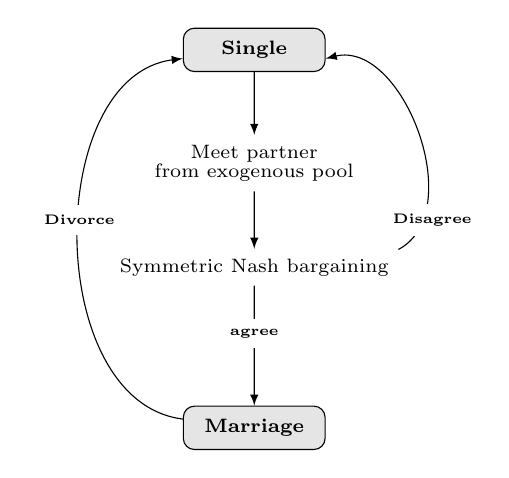
\begin{tikzpicture}[domain=0:1,scale=1.2]

%From below: cohabitation and marriage
\node [re1] at (2.25,+0.0) (ma) {\scriptsize\bf Marriage}  ;
%\node [re1] at (+4.5,+0.0) (co) {\scriptsize\bf Cohabitation};

%Single plus procedure
\node [re1] at (+2.25,+4.0) (si) {\scriptsize\bf Single};

\node [re2] at (+2.25,+2.8) (me) {\scriptsize Meet partner\\ \scriptsize from exogenous pool};
\node [re2] at (+2.25,+1.7) (na) {\scriptsize  Symmetric Nash bargaining};

%\node [re3] at (+0.0,+4.0) (di) {\scriptsize\bf Divorce};
%\node [re3] at (+4.5,+4.0) (br) {\scriptsize\bf Breakup};


\draw [->,>=latex] (si) -- (me);
\draw [->,>=latex] (me) -- (na);
%\draw [->] (na) -- (ma);
%\draw [->] (na) -- (co);
%\draw [->,>=latex] (ma) -- (di);
%\draw [->,>=latex] (co) -- (br);
%\draw [->,>=latex] (di) -- (si);
%\draw [->,>=latex] (br) -- (si);
%\draw [->,>=latex] (co) -- (ma);

\draw [->,>=latex] (na) to [bend right=83] (si);

\draw [->,>=latex] (na) to  (ma);
\draw [->,>=latex] (ma) to [bend left=83] (si);


\node [re4] at (+3.8,+2.2) (dis) {\tiny \bf \quad \quad \quad Disagree};

\node [re4] at (+0.4,+2.2) (dis) {\tiny \bf Divorce};

\node [re4] at (+2.25,+1.0) (ag) {\tiny \bf agree};

\end{tikzpicture}



